\chapter{Logica di Floyd-Hoare}

Lo scopo della \fancyglitter{verifica dei programmi} è il controllo della soddisfacibilità delle specifiche, ossia che il programma sia \fancyglitter{corretto} e \fancyglitter{compilante}. Negli anni '60 Floyd propose di inserire delle formule logiche nei flow-chart dei programmi e Hoare introdusse le \fancyglitter{triple}\footnote{Accennate nel capitolo precedente.}.

\begin{center}
 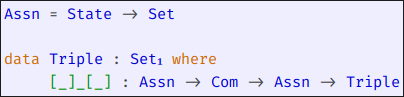
\includegraphics[scale = 0.5]{images/IMP/Assn.png}
\end{center}

\nt{Il tipo \texttt{Set}$_1$ è l'\fancyglitter{universo} più piccolo tale che \texttt{Set} = \texttt{Set}$_0$ : \texttt{Set}$_1$.}

\section{Il sistema della logica di Hoare}

\dfn{Logica di Hoare}{
  La logica di Hoare è un'assiomatizzazione della nozione di correttezza parziale. Consiste di un sistema formale di regole di inferenza i cui giudizi sono triple più formule logiche.
}

\subsection{Regole}

\begin{center}
 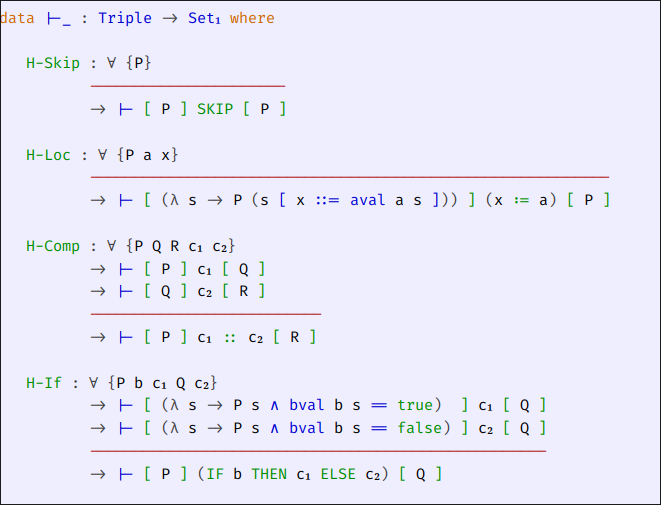
\includegraphics[scale = 0.4]{images/IMP/T1}
\end{center}

\begin{center}
 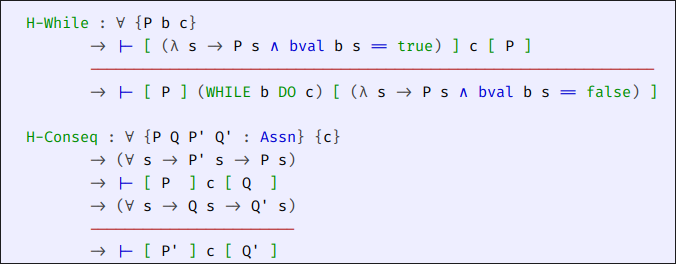
\includegraphics[scale = 0.4]{images/IMP/T2}
\end{center}

\nt{Per via della nostra definizione di asserzione ci sono alcune differenze con le regole originali.}

\subsection{Regole derivate}


\begin{center}
 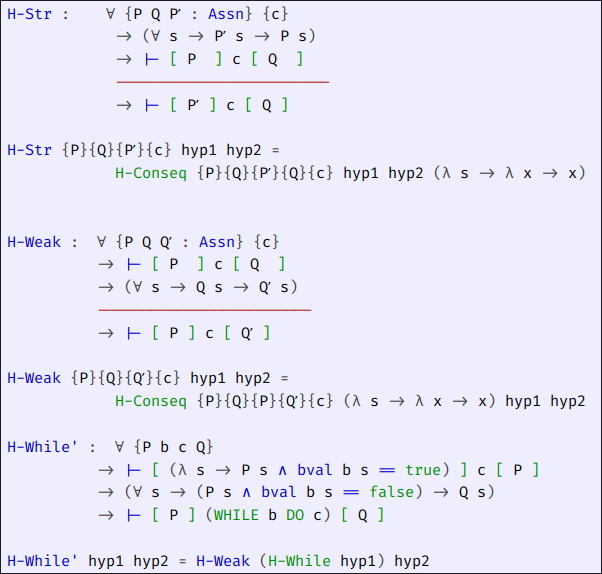
\includegraphics[scale = 0.4]{images/IMP/T3}
\end{center}

\section{Esempi}

\subsection{Assegnamento}

\begin{center}
 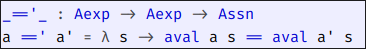
\includegraphics[scale = 0.6]{images/IMP/Ug}
 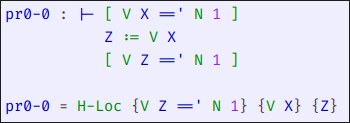
\includegraphics[scale = 0.6]{images/IMP/pr0-0}
 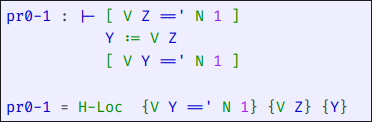
\includegraphics[scale = 0.6]{images/IMP/pr0-1}
\end{center}

\nt{La pre-condizione X = 1 è il risultato della sostituzione di Z con X nella post-condizione Z = 1. Dato che il comando termina sempre e assegna il valore di X a Z la tripla è valida (secondo il nostro formalismo \fancyglitter{H-Loc}).}

\subsection{Composizione}

\begin{center}
 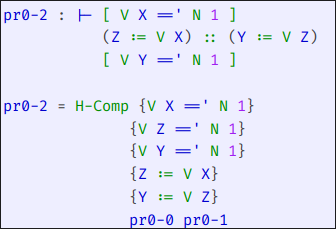
\includegraphics[scale = 0.6]{images/IMP/pr0-2}
\end{center}

\nt{Basta applicare la regola \fancyglitter{H-Comp} a pr0-0 e pr0-1.}

\subsection{Selezione}

Consideriamo \{T\} IF X $<$ Y THEN Z := Y ELSE Z := X \{Z = max(X,Y)\}\{T\} IF X $<$ Y THEN Z := Y ELSE Z := X \{Z = max(X,Y)\} (T è sempre vera, triviale). Per dimostrarla dobbiamo prima dimostrare:

\begin{center}
  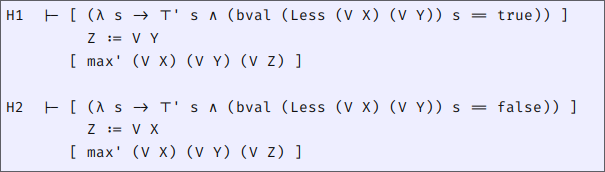
\includegraphics[scale = 0.5]{images/IMP/Ipotesi}
\end{center}

\begin{center}
  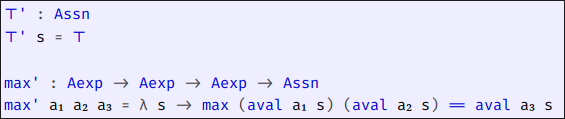
\includegraphics[scale = 0.5]{images/IMP/T-max}
\end{center}

\nt{max è $\bbN \to \bbN \to \bbN$ ed è definita nella libreria Nat.agda.}

\begin{center}
  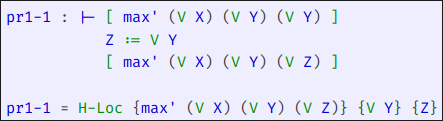
\includegraphics[scale = 0.4]{images/IMP/pr1-1}
  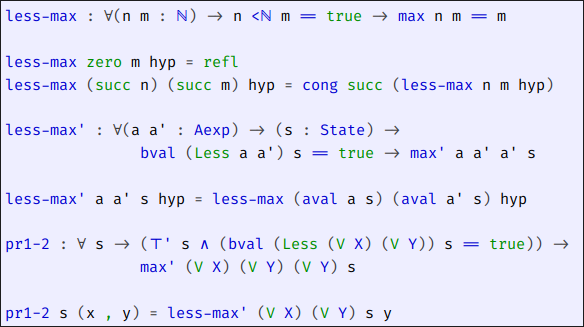
\includegraphics[scale = 0.4]{images/IMP/pr1-2}
\end{center}

\nt{Ora si può provare H1 mediante la regola di rafforzamento (\fancyglitter{H-STR}).}

\begin{center}
  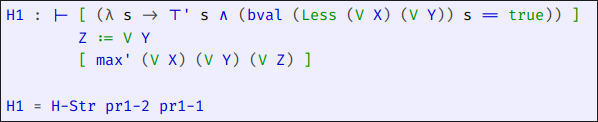
\includegraphics[scale = 0.5]{images/IMP/H1}
\end{center}

\nt{In maniera simile possiamo provare H2.}


\begin{center}
  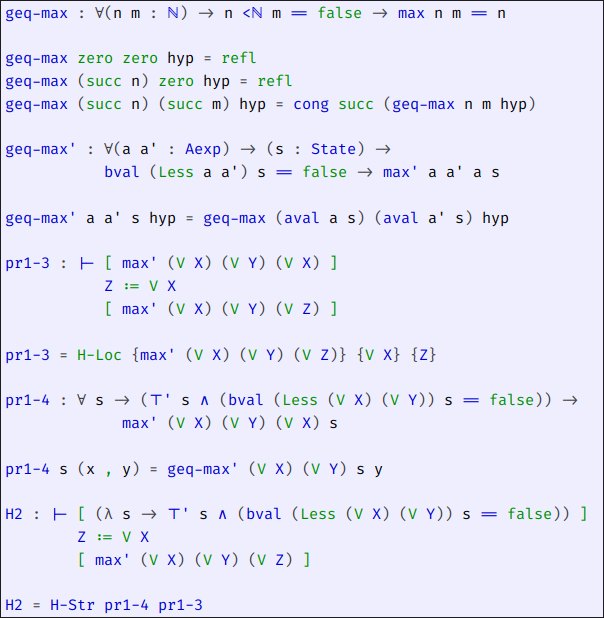
\includegraphics[scale = 0.5]{images/IMP/H2}
\end{center}

\nt{Infine si applica \fancyglitter{H-IF} alle ipotesi.}


\begin{center}
  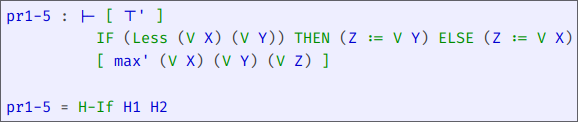
\includegraphics[scale = 0.5]{images/IMP/pr1-5}
\end{center}

